

\section{Outline}
This chapter will discuss the analysis of PGGs on networks using the model developed by Marco Tomassini and Alberto Antonioni in \cite{RN49}. First, their model is replicated, and the replicated results are compared to the published results. Then the replicated results are examined for robustness. After that, the analysis is extended to further graph types to analyse the effect of graph structure on cooperation. Under the Tomassini--Antonioni model, network models with high clustering coefficient $C_\Delta$ induce lower cooperation for low values of $r$ and higher cooperation for higher values of $r$ relative to models with low $C_\Delta$, regardless of degree size distribution. \\

\section{Payoff Satisfaction Model}
This model described in \cite{RN49} emulates an agent who increases their contribution when they are \emph{satisfied}. That is, their total return from the common pools are greater than their contributions. The goal of the \emph{satisfaction} model is to accurately reflect results observed in human experiments. This differs strongly from evolutionary dynamics, which will be discussed in a later chapter. The payoff $\pi_i$ of an individual $i$ enrolled in $g_i$ groups each with size $|N_j|$ is \\
\begin{align} \label{TA_pi}
    \pi_i(c_i) = - g_ic_i + \sum_{j=1}^{g_i} \sum_{k=1}^{|N_j|} \frac{rc_k}{|N_j|}, \quad c_i \in C:= \{0.0, 0.25, 0.50, 0.75, 1.0\}. 
\end{align}

It is enforced that each player contributes a constant $c_i$ to each group, and is initially endowed with $g_i$ units. The first term of \eqref{TA_pi} their contribution, and the last term represents the return earned from all the games, enhanced by $r$. \\

Each agent's initial contribution is randomly chosen from the set $C$. The choice set qualitatively emulates a lab experiment, where players are given tokens and choose how many tokens to contribute. \\

The agents' update rule is simple. If they receive, from the common pools, at least as much as they contribute, they are \emph{satisfied}. That is, an agent is \emph{satisfied} when $\sum_{j=1}^{g_i} \sum_{k=1}^{|N_j|} \frac{rc_k}{|N_j|} - g_i c_i\geq g_i c_i$. In this case, they increase their contribution by 0.25 with probability 0.5, otherwise remain unchanged. If they are \emph{unsatisfied}, their contribution always decreases by 0.25. Obviously an agent playing $c_i =1$ cannot increase their contribution, and similarly an agent playing $c_i=0$ cannot decrease their contribution. This model does not claim to simulate evolutionary dynamics, instead it intends to replicate results observed in human trials. \\


\section{Network Structure}
Antonioni and Tomassini developed their own model for the generation of social networks in the paper \cite{RN51}. This model considers the degree of vertices as well as their location in two-dimensional unitary space $[0,1]^2$. Similar to the Barab\'{a}si--Albert model described in \ref{BA}, a growing mechanism is used to create the graph. The parameters are  the population size $N$, the targeted mean degree, $m$, and  a mixing parameter, $\alpha$. \\

The graph is initialised with a clique of $m+1$ nodes distributed in $[0.45, 0.55]^2$. Then each new node is added randomly in $[0,1]^2$ and prescribed a number of links drawn from $\mathsf{DU}(1,2m-1)$. For each link, a uniform random number is compared to the parameter $\alpha$. If the random number is less than $\alpha$, the node is then joined to an existing node chosen by preferential attachment as in a Barab\'{a}si--Albert model. Otherwise, the node is joined to the geometrically closest existing node that is not already linked. \\

The paper \cite{RN51} compares graphs built using this model to real-world graphs, and finds it exhibits the common features for a social network. Relative to a Barab\'{a}si--Albert model, the clustering coefficient is higher due to the spatial dimension. It also preserves the right-skewed degree distribution and low path lengths. \\

This network model serves as the structure for the game in \cite{RN49}, with agents stationed at nodes. For each figure, the simulation has parameters $N=500, m = 6, T=100$, where $T$ represents the number of trials for each parameter combination. The plotted series represents the mean taken over all $T$ trials. In \cite{RN49}, Tomassini and Antonioni also used $N=500, m = 6$. \\

\section{Results Comparison}
The results obtained by simulation were compared to the results reported in the paper \cite{RN49}. The comparison is shown in Figure \ref{comp0}. \\

\FloatBarrier 
\begin{figure}[!h]
  \begin{subfigure}[b]{0.45\textwidth}
    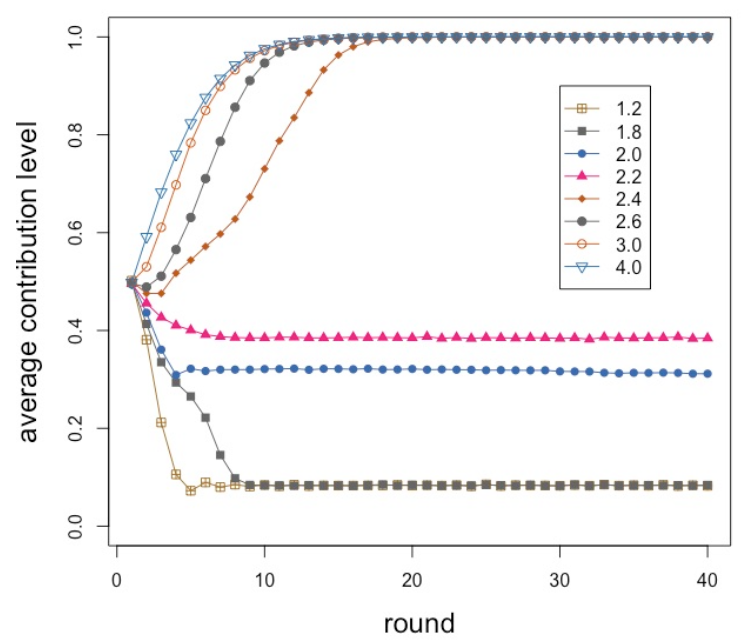
\includegraphics[width=\textwidth]{images/TAfig2_real.png}
    \caption{Figure 2 from \cite{RN49}. }
    \label{TAfig2_real}
  \end{subfigure}
  \hfill
  \begin{subfigure}[b]{0.45\textwidth}
    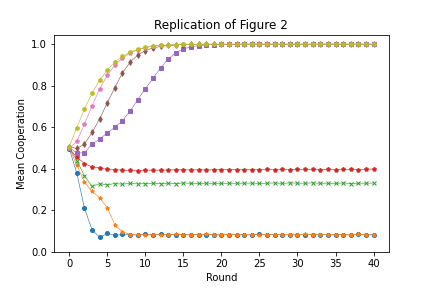
\includegraphics[width=1.25\textwidth]{images/TAfig2.png}
    \caption{Replication of \ref{TAfig2_real}. }
    \label{TAfig2}
  \end{subfigure}
  \caption{Comparison of reported results from \cite{RN49} and replicated results. Each series represents a value for the enhancement factor $r \in \{1.2, 1.8, 2.0, 2.2, 2.4, 2.6, 3.0, 4.0\}$, which correspond to blue circles, orange stars, green crosses, red pentagons, purple squares, brown diamonds, pink pentagons, and olive hexagons respectively. The simulation is identical to the reported results, indicating that the replication is successful. The mixing parameter $\alpha$ was set to 0.3.} \label{comp0}
\end{figure} 
\FloatBarrier

Evidently, increasing the enhancement factor $r$ increases cooperation. It is interesting to note that equilibrium is reached relatively quickly ($\sim$ 20 rounds). In \cite{RN49}, the authors note that even in the case of low $r$, zero cooperation is not observed. This agrees with experimentally reported results, but disagrees with classical and evolutionary game theory predictions. In fact, the minimum contribution amount of 0.0833 can be shown analytically as a steady state under some simplifying assumptions.\\


\newtheorem{lemma_mcb}[theorem]{Lemma} \label{mcb}
\begin{lemma_mcb}
In the \emph{satisfaction} model, under mean-field assumptions and for enhancement factor $r \geq0$, there exists a population minimum contribution bound $\Bar{c} = \tfrac{1}{12}.$ such that any equilibrium contribution $c^*$ achieves at least $\Bar{c}$.  \end{lemma_mcb}
\begin{proof}
Consider a representative agent $i$. By the mean-field assumption, they are enrolled in $g=7$ games, each with $7$ agents per game. Also assume each interacting agent is contributing at the population equilibrium proportion $c^*$. If agent $i$ is playing $c_i = 0$, then their payoff is \\
\begin{equation}
    \pi_i(0, c^*)= \mathbb E - gc_i + \sum_{j=1}^{g_i} [\sum_{k=1}^{|N_j|} \frac{rc_k}{|N_j|}] =   7\times\frac{6rc^* + 0r}{7}-7\times0 \geq 7\times0, \quad \forall r, c^* \geq 0.
\end{equation}
So agent $i$ will be satisfied, and therefore increase their contribution to 0.25 with probability $\tfrac{1}{2}$ or else keep $c_i = 0$ in the next step. \\

To find the minimum contribution bound, assume that agent $i$ is unsatisfied with their contribution if $c_i = 0.25$. Otherwise their contribution $c_i$, and hence the equilibrium contribution $c^*$ will be greater than 0.25 and the minimum contribution bound will be achieved. 

The payoff for agent $i$ of $c_i$ is  \\
\begin{equation} \label{unsat}
    \pi_i(0.25, c^*)= \mathbb E - gc_i + \sum_{j=1}^{g_i} [\sum_{k=1}^{|N_j|} \frac{rc_k}{|N_j|}]  =   7\times\frac{6rc^* + 0.25r}{7}-7\times0.25. 
\end{equation}
For agent $i$ to be unsatisfied at this level, it holds that $\pi_i(0.25, c^*) <7\times 0.25$. So $r,c^*$ solve $7\times\frac{6rc^* + 0.25r}{7}<14\times0.25$. If agent $i$ is unsatisfied, then they decrease their contribution to 0. This is a Markov process for the states 0, 0.25. The transition matrix $\mathbf{P}$, is $$\mathbf P = \begin{bmatrix} 0.5& 0.5 \\
1& 0 \\
\end{bmatrix}. $$  Equilibrium is achieved when the Markov process is stationary. The stationary distribution solves $\pi \mathbf{P} = \pi$. For $\mathbf{P}$ defined above, $\pi = [\tfrac{2}{3}, \tfrac{1}{3}]$, which corresponds to a mean contribution of $\tfrac{1}{12} =\Bar{c}$. Hence for any $r$, the minimum contribution is at least $\Bar{c}$. \\
\end{proof}

An implication of \eqref{unsat} is that $\Bar{c}$ is an equilibrium for $r<4.67$. Yet only the trends corresponding to $r<2$ achieve the minimum contribution bound. This is because there are other equilibria between $c^*=0.5$ and $\Bar{c}$ that are achieved for $r\geq2$. By varying the initial conditions, different values of $r$ can achieve the minimum contribution bound. \\

 The analytical result of $\tfrac{1}{12}$ and the numerical result for the trend $r=1.8$ differ by 0.0002. In the context of a simulation comprised of 500 agents, this indicates the numerical result differs from the analytical prediction by approximately one agent every ten simulations. This could be due to the stochastic nature of the simulations, or the effect of the simplifying assumptions. \\



For further confirmation, Figures 5a and b from the paper were also replicated, shown in Figures \ref{comp1}, and \ref{comp2}. These correspond to modifying the underlying graph to a purely spatial ($\alpha = 0$), or preferential attachment ($\alpha = 1)$ model. The similarity of these results indicates both the agent and graph models correctly replicate the descriptions given in \cite{RN49}.

\FloatBarrier
\begin{figure}[!h] 
  \begin{subfigure}[b]{0.45\textwidth}
    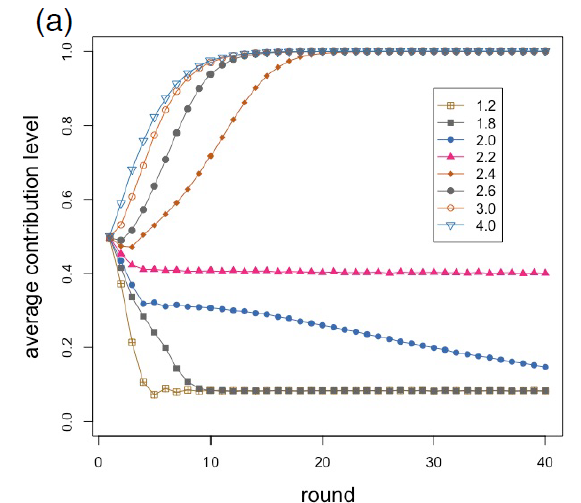
\includegraphics[width=\textwidth]{images/TAfig4a_real.png}
    \caption{Figure 5a from \cite{RN49}. $\alpha = 0$ }
    \label{TAfig4a_real}
  \end{subfigure}
  \hfill
  \begin{subfigure}[b]{0.45\textwidth}
    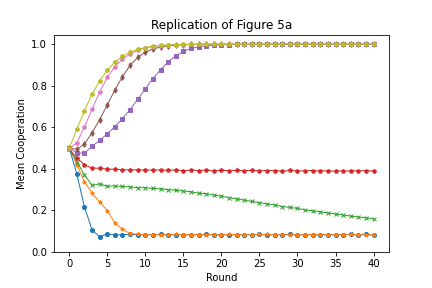
\includegraphics[width=1.35\textwidth]{images/TAfig4a.png}
    \caption{Replication of \ref{TAfig4a_real}. }
    \label{TAfig4a}
  \end{subfigure}
  \caption{Comparison of reported results from \cite{RN49} and replicated results. Each series represents a value for the enhancement factor $r \in \{1.2, 1.8, 2.0, 2.2, 2.4, 2.6, 3.0, 4.0\}$, which correspond to blue circles, orange stars, green crosses, red pentagons, purple squares, brown diamonds, pink pentagons, and olive hexagons respectively. Once again, the replication is successful.  Mixing parameter $\alpha = 0.0$. } \label{comp1}
\end{figure} 
\FloatBarrier




\FloatBarrier
\begin{figure}[!h] 
  \begin{subfigure}[b]{0.45\textwidth}
    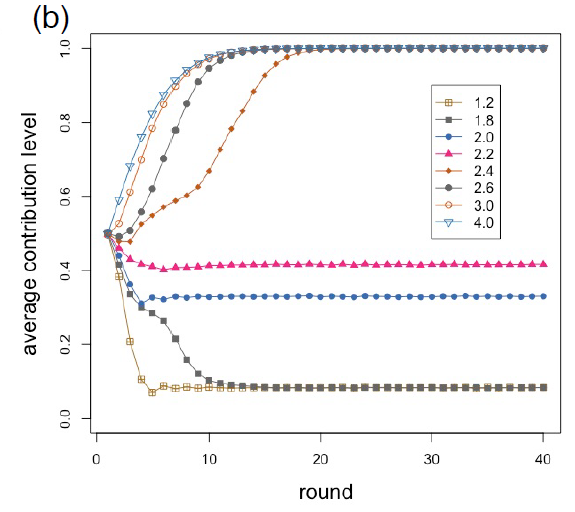
\includegraphics[width=\textwidth]{images/TAfig4b_real.png}
    \caption{Figure 5b from \cite{RN49}. $\alpha = 1$ }
    \label{TAfig4b_real}
  \end{subfigure}
  \hfill
  \begin{subfigure}[b]{0.45\textwidth}
    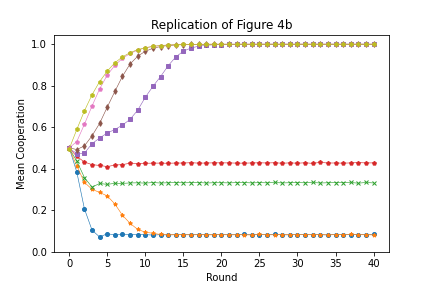
\includegraphics[width=1.35\textwidth]{images/TAfig4b.png}
    \caption{Replication of \ref{TAfig4b_real}. }
    \label{TAfig4b}
  \end{subfigure}
  \caption{Comparison of reported results from \cite{RN49} for $\alpha = 1$. Each series represents a value for the enhancement factor $r \in \{1.2, 1.8, 2.0, 2.2, 2.4, 2.6, 3.0, 4.0\}$, which corresponds to blue circles, orange stars, green crosses, red pentagons, purple squares, brown diamonds, pink pentagons, and olive hexagons respectively. The replication is again successful. } \label{comp2}
\end{figure} 
\FloatBarrier

The key results from \cite{RN49} have been reproduced. Because the results were replicated for varying graph parameter $\alpha$, and model parameter $r$, then the implementation of the model and network structure mirrors \cite{RN49}. Other results from their paper, where the mean degree is varied, have also been reproduced, but are not included for the sake of brevity.\\


\section{Robustness}
The robustness of results was discussed qualitatively in \cite{RN49}, and the authors demonstrated consistency in results. However no quantitative analysis was provided. To examine the robustness of the results, the empirical quantiles, as well as the confidence interval for the mean of each series, are examined. The first plot examines the shape of the distribution for each of the series by plotting the empirical 2.5\% and 97.5\% quantiles. \\

\FloatBarrier
\graphCap{sensitivity2.pdf}{0.8}{2.5\% and 97.5\% quantiles for each series. Each series represents a value for the enhancement factor $r \in \{1.2, 1.8, 2.0, 2.2, 2.4, 2.6, 3.0, 4.0\}$, which corresponds to blue circles, orange stars, green crosses, red pentagons, purple squares, brown diamonds, pink pentagons, and olive hexagons respectively. The mean is shown as a solid line, and the quantiles as dashed. Only 5 out of 100 trials lie outside the dashed lines for each series.}{sens2}
\FloatBarrier
The series corresponding to $r=2.2$ shows a 97.5\% quantile trend of around 0.58. This is much higher than the mean trend. This shows the influence of the particular network within the network model, particularly for the critical values at which cooperation is sustained but full cooperation is not achieved. It is interesting to note that this phenomenon does not occur for the $r=2$ line, which also achieves incomplete but non-zero cooperation. A granular simulation was carried out for $r \in [2.0,2.5]$, and it was found that for $r \in [2.2, 2.28]$, the 2.5\% quantile is the same, however the mean trends are different. There appears to be a lower bound of 0.33 for $r \in [2.0, 2.5]$, which represents a population switching between 0.25 and 0.5 similar to the lower bound of 0.0833 discussed in reference to Lemma \ref{mcb}.\\

Figure \ref{sens1} applies the Central Limit Theorem to the cooperation level, and plots a $95\%$ confidence interval for the mean for each series. The Central Limit Theorem derives a 95\% CI for the mean, as $\hat{\mu} \pm 1.96\times\frac{\hat{\sigma}}{\sqrt{T}}$, where $\hat{\sigma}$ is the empirical standard deviation. The Central Limit Theorem is applicable, as there are more than 30 samples for each series. \\
\FloatBarrier
\graphCap{sensitivity1.pdf}{0.8}{95\% Confidence interval for the mean of each series. Each series represents a value for the enhancement factor $r \in \{1.2, 1.8, 2.0, 2.2, 2.4, 2.6, 3.0, 4.0\}$, which corresponds to blue circles, orange stars, green crosses, red pentagons, purple squares, brown diamonds, pink pentagons, and olive hexagons respectively. The mean is shown in the solid line, and the bounds of the confidence interval are shown as dashed lines. It is evident that the results are stable. Only the middle series, $r=2.2$, shows some variance.}{sens1}
\FloatBarrier
Figure \ref{sens1} shows that the means are stable, and the results are robust. The confidence intervals for the mean are symmetric about the mean, due to the assumption of limiting normality. \\

To investigate the effect of network structure on cooperation, the Tomassini--Antonioni model will be extended to other network models. \\

\section{Extension to Other Network Models} \label{other_networks}

In \ref{RG}, three main network models are discussed. These are the Erd\H{o}s--R\'enyi graph, \emph{small-world} network (Watts--Strogatz, WS), and also the Barab\'{a}si--Albert (BA) model. In the following analysis, $G(n,r)$ graphs are chosen for Erd\H{o}s--R\'enyi graphs, and denoted RRG (random regular graphs). This is to be able to control the mean degree. All three of these network models are implemented using the \verb+networkx+ Python package. For comparison, the model described by Tomassini and Antonioni in \cite{RN51} is included, and denoted Tomassini Antonioni Graph (TAG). Across all graphs, the targeted mean degree, $m$, is set to 6 to allow comparison between graph models. \\

Small-world networks describe a family of graphs, depending on the parameter $p$. For this analysis, $p$ was set to 0.1, which preserves local clustering and reduces the average shortest path length. Importantly, only connected WS graphs are used. If the graph generated is not connected, then a new one with the same parameter is generated until they are connected. This is convention to allow strategies to propagate throughout the graph. \\

Similarly, TAG is a family of graphs. In the plots below, the proportion parameter $\alpha$ is set to 0.3, as recommended by \cite{RN49}.\\

For clarity, a sample of 100 graphs for each model were taken, and their descriptive statistics computed. The targeted mean degree $m$ is set to 6, and the graph size, $N$ is set to 500. \\


\FloatBarrier

    

\begin{table}[!h]
\begin{center}
\begin{tabular}{|l|l|l|l|l|}
\hline
Graph Type & Mean Degree & $l$ & $C_\Delta$ & Degree Variance \\ \hline
BA         & 5.96        & 3.24                         & 0.05                   & 40.80           \\ \hline
RRG        & 6           & 3.75                         & 0.01                   & 0               \\ \hline
TAG        & 5.99        & 3.84                         & 0.22                   & 16.95           \\ \hline
WS         & 6           & 5.39                         & 0.44                   & 0.57            \\ \hline
\end{tabular}
\caption{Computed characteristics for BA, RRG, TAG, and WS models. The characteristics were computed over 100 samples of each graph, and then averaged. The WS entry considers a connected WS graph with $p=0.1$. The TAG entry considers a TAG graph with $\alpha = 0.3$. } \label{graph_stats}
\end{center}
\end{table}

\FloatBarrier

The degree variance does not accurately describe all the facets of the degree distribution, so a histogram for each model is plotted below. For each graph model, 100 graphs were created according to the previously described parameters and their degree counts summed to create the histograms. \\
\FloatBarrier
\graphCap{hist1.pdf}{0.7}{Degree Histogram for WS and RRG models. The RRG model enforces a degree of 6 for every node. The WS model starts from a lattice, then rewires each link with probability $p=0.1$.}{hist1}
\FloatBarrier
\graphCap{hist2.pdf}{0.7}{Degree Histogram for BA and TAG models, on a logarithmic scale. The logarithmic scale clearly shows the counts for higher degrees. Because the TAG model only uses preferential attachment $\alpha = 0.3$ proportion of the time, it is not a true scale-free distribution. }{hist2}
\FloatBarrier
One of the goals of the TAG is to preserve a higher clustering coefficient than BA graphs, while remaining approximately scale-free. Table \ref{graph_stats} emphasises this effect. From these descriptive statistics, it appears that BA and RRG can be considered similar except for their degree distributions. The mean cooperation level for each graph was plotted. Because this is novel analysis, each trial observes 60 steps. \\


\FloatBarrier
\graphCap{graphs1.pdf}{0.8}{Comparing network models, $r \in \{1.8, 1.85, 1.9, 1.95\}$. In each graph, the blue circles, orange stars, green crosses, and red pentagons correspond to the WS model, TAG model, BA model, and RRG model respectively. It is observed that first RRG, then BA, then TAG, then WS achieve non-trivial cooperation. This corresponds to the order of increasing $C_\Delta$. }{graphs1}
\FloatBarrier

It appears that $C_\Delta$ dictates the value for $r$ for which non-trivial cooperation is observed. Interestingly, for $\alpha = 0.3$, 30\% of the TAG graph are nodes added in BA style. Yet the TAG graph reflects the trend of the WS model more than the BA model.
\FloatBarrier
\graphCap{graphs2.pdf}{0.8}{Comparing Graph models, $r \in \{2.0,2.05,2.1,2.15\}$. In each graph, the blue circles, orange stars, green crosses, and red pentagons correspond to the WS model, TAG model, BA model, and RRG model respectively. For $2.0<r<2.25$, the cooperation levels are very similar around 0.33, and the WS model requires the highest enhancement factor $r$ to achieve non-trivial cooperation.  \\ }{graphs2}
\FloatBarrier
\graphCap{graphs3.pdf}{0.8}{Comparing Graph models, $r \in \{2.2, 2.25, 2.3, 2.35\}$. In each graph, the blue circles, orange stars, green crosses, and red pentagons correspond to the WS model, TAG model, BA model, and RRG model respectively. For $2.0<r<2.25$, the cooperation levels were very similar around 0.5, so the plots are not shown.  It is an almost perfect trend reversal, as WS is the first graph to achieve full cooperation, then TAG, then BA and finally RRG. For $r>2.35$, full cooperation was always achieved. \\ }{graphs3}
\FloatBarrier
For the range of $r$ in Figure \ref{graphs3}, it is more interesting. The WS and TAG trends achieve full cooperation earlier. This seems to indicate that the agents are more uniform under this graph structure. The WS and TAG models have a small range of $r$ for which non-trivial cooperation is observed. These graph models also have high $C_\Delta$, which may propagate strategies through the population, and enforce homogeneity in contribution. Both the WS and RRG model have very low degree variance, yet behave quite differently. It appears that the degree distribution does not impact the cooperation level for Tomassini--Antonioni style agents. \\

\section{Summary}

This chapter focused exclusively on agents defined by Tomassini and Antonioni in \cite{RN49}. Tomassini and Antonioni demonstrated that these agents are a good proxy for human interactions, and simulated the Public Goods Game on a custom network model. These results were perfectly replicated, and both plots are shown in Figures \ref{comp0}, \ref{comp1}, and \ref{comp2}.  A lower bound for cooperation of 0.0835 was demonstrated analytically. The robustness of these results were also examined. It is shown that 100 repetitions were sufficient to estimate the mean of each series, however the empirical quantile plots showed that there is quite high variance in distribution for the series corresponding to $r=2.2$.\\ 

The agents from this model were then tested on different models for random graphs. The results are interesting in the range $1.85\leq r \leq 2.4$. The trend indicates that models with high clustering coefficient $C_\Delta$ do not support intermediate levels of cooperation, and remain at the lower bound of cooperation for higher $r$ and full cooperation for lower $r$ relative to models with low $C_\Delta$. Other characteristics of the graph model, such as the distribution of node size, and $l$, did not seem to have an effect. \\



